%
% polynom.tex
%
% (c) 2020 Prof Dr Andreas Müller, Hochschule Rapeprswil
%
\section{Interpolationspolynom
\label{buch:section:interpolationspolynom}}
\rhead{Lagrange-Interpolationspolynome}
In diesem Abschnitt wird das folgende Problem gelöst.
\begin{aufgabe}[Interplations-Polynom]
Gegeben Stützstellen
\[
a=x_0<x_1<x_2<\dots < x_{n-1}<x_n=b
\]
und Funktionswerte $f_i, 0\le i\le n$, finde ein Polynome $l(x)$
mit der Eigenschaft $l(x_i)=f_i$ für alle $i=0,1,\dots n$.
\end{aufgabe}
Gegeben sind also $n+1$ Bedingungen, die das Polynom erfüllen muss.
Abgesehen von trivialen Fällen wie dem Null-Polynom, muss ein Polynom
im Allgemeinen mindestens den Grad $n$ haben, damit alle 
Bedingungen durch geeignete Wahl der $n+1$ Koeffizienten erfüllt werden können.
Man könnte das Polynom nämlich in der Form
\[
p(x)
=
a_nx^n + a_{n-1}x^{n-1}+\dots+a_1x+a_0
\]
ansetzen und die Stützstellen einsetzen.
Lösung des Gleichungssystem
\begin{equation}
\begin{linsys}{5}
a_Nx_0^N &+& a_{N-1}x_0^{N-1} &+& \dots &+& a_1x_0 &+& a_0x_0 &=& f_0 \\[5pt]
a_Nx_1^N &+& a_{N-1}x_1^{N-1} &+& \dots &+& a_1x_1 &+& a_0x_1 &=& f_1 \\[5pt]
\vdots   & &    \vdots        & & \ddots& & \vdots & & \vdots & & \vdots\\[5pt]
a_Nx_n^N &+& a_{N-1}x_n^{N-1} &+& \dots &+& a_1x_n &+& a_0x_n &=& f_n 
\end{linsys}
\end{equation}
liefert dann die gesuchten Koeffizienten.
Dieser Weg ist allerdings sehr aufwendig, die Lösung eines linearen
Gleichungssystems mit dem Gauss-Algorithmus benötigt $O(n^3)$ Operationen.
Die sehr spezielle Struktur des Gleichungssystems sollte ermöglichen,
das Polynom $l(x)$ auf direkterem Weg zu ermitteln.

%
% Interpolationspolynom bestimmen
%
\subsection{Bestimmung des Interpolationspolynoms
\label{buch:section:interpolation:bestimmung}}
Das allgemeine Interpolationsproblem kann leicht gelöst werden, wenn
das folgende spezielle Interpolationsproblem gelöst ist.

\begin{aufgabe}[Spezielle Interpolationspolynome]
\label{buch:aufgabe:speziellesinterpolationsproblem}
Gegeben die Stützstellen
\[
a=x_0<x_1<x_2<\dots <x_{n-1}<x_n=b,
\]
finde Polynome $l_j$ vom Grad $n$ derart, dass
\[
l_j(x_i) = \delta_{ij}=\begin{cases}
1&\qquad i=j\\
0&\qquad\text{sonst.}
\end{cases}
\]
\end{aufgabe}

\begin{figure}
\centering
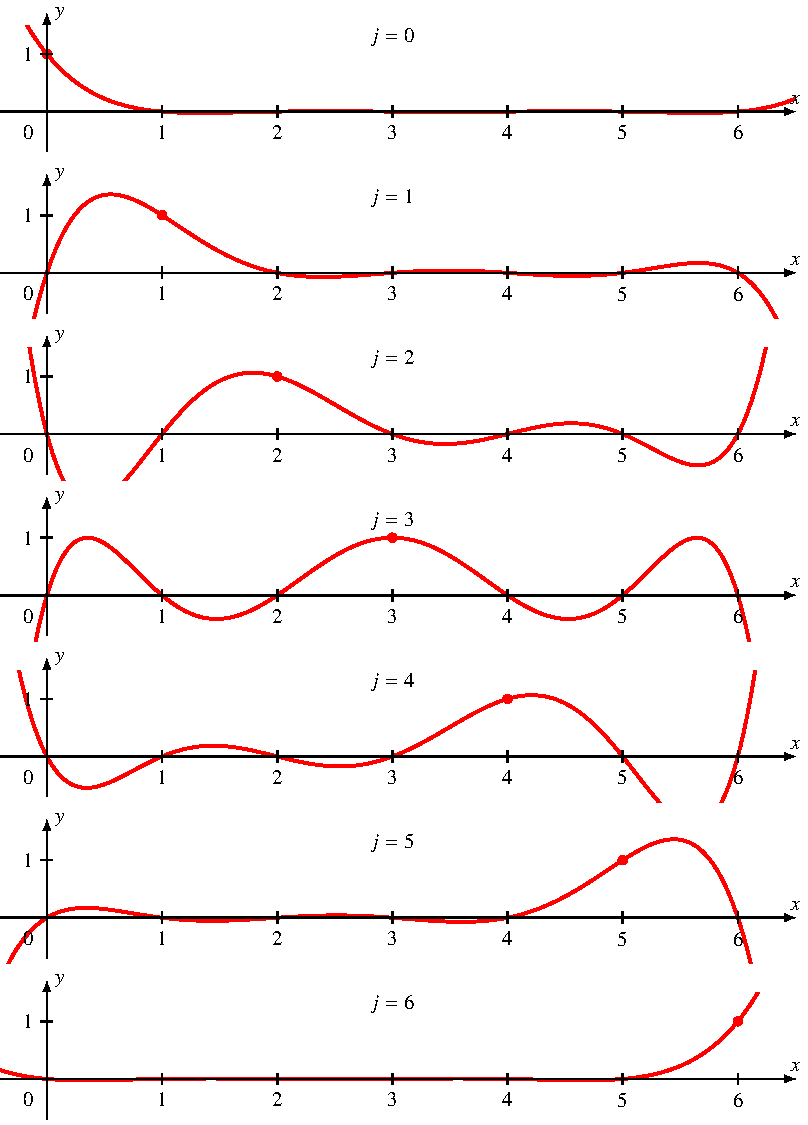
\includegraphics{chapters/30-interpolation/figures/basis.pdf}
\caption{Polynome $l_j(x)$, welche des spezielle Interpolationsproblem
\ref{buch:aufgabe:speziellesinterpolationsproblem}
lösen.
\label{buch:figure:spezielleinterpolation}}
\end{figure}

Jedes der Interpolationspolynome $l_j$ hat Grad $n$, also hat auch eine
beliebige Linearkombination den Grad höchstens $n$.
Die Linearkombination
\[
p(x) = \sum_{j=0}^n f_j l_j(x)
\]
ist das gesuchte Interpolationspolynom, wie Einsetzen von $x_i$ in
\[
p(x_i)
=
\sum_{j=0}^n f_jl_j(x_i)
=
\sum_{j=0}^n f_j\delta_{ij}
=
f_i
\]
bestätigt.

\begin{beispiel}
Ein besonders einfacher Fall ist $n=1$.
Gesucht ist eine lineare Funktion $l(x)=a_1x+a_0$ derart, dass
$l(x_0)=f_0$ und $l(x_1)=f_1$.
Polynome $l_0$ und $l_1$ können leicht angegeben werden:
\[
l_0(x) = \frac{x_1-x}{x_1-x_0}
\qquad\text{und}\qquad
l_1(x) = \frac{x-x_0}{x_1-x_0}
\]
haben die die geforderten Eigenschaften.
Die gesuchte Interplationsfunktion ist daher
\[
p(x)
=
\frac{x_1-x}{x_1-x_0}f_0 + \frac{x-x_0}{x_1-x_0} f_1
=
x \frac{f_1-f_0}{x_1-x_0}   + \frac{x_1f_0-x_0f_1}{x_1-x_0}.
\]
Der Koeffizient von $x$ ist wie erwartet die Steigung der Geraden durch
die Punkte $(x_0,f_0)$ und $(x_1,f_1)$.
\end{beispiel}

Ein Polynom vom Grad $n+1$, welches in {\em allen} Stützstellen verschwindet,
ist leicht zu finden, es ist 
\[
(x-x_0)(x-x_1)(x-x_2)\cdots (x-x_{n-1})(x-x_n).
\]
Ein Polynom, welches nur an der Stützstelle $x_j$ {\em nicht} verschwindet,
ensteht, indem man den Faktor $(x-x_j)$ weglässt, es hat den Grad $n$.
Wir führen dafür die Notation
\[
(x-x_0)(x-x_1)(x-x_2)\cdots \widehat{(x-x_j)}\cdots (x-x_{n-1}(x-x_n),
\]
der Hut bedeutet, dass dieser Faktor weggelassen werden soll.
Allerdings hat dieses Polynom nicht den geforderten Wert $1$, man muss es
also noch mit einer geeigneten Konstante multiplizieren.
Das gesuchte Polynom $l_j(x)$ hat daher die Form
\[
l_j(x)
=
c_j(x-x_0)(x-x_1)(x-x_2)\cdots \widehat{(x-x_j)}\cdots (x-x_{n-1}(x-x_n).
\]
Einesetzen von $x_j$ ergibt
\[
l_j(x_j) = 1 = 
c_j(x_j-x_0)(x_j-x_1)(x_j-x_2)\cdots \widehat{(x_j-x_j)}\cdots(x_j-x_{n-1})(x_j-x_n),
\]
die Konstante $c_j$ ist daher
\[
c_j = \prod_{i=0\atop i\ne j}^n \frac{1}{x_j-x_i}.
\]

\begin{beispiel}
Man finde ein Polynome, welches $l(0)=l(1)=0$ und $l(\frac12)=1$
erfüllt.
Wegen $f_0=f_2=0$ ist nur das Polynome $l_1$ zu ermitteln, es ist
\[
l(x) = l_1(x)
=
\frac{(x-x_0)(x-x_2)}{(x_1-x_0)(x_1-x_2)}
=
\frac{x(x-1)}{\frac12(\frac12-1)}
=
\frac14x(1-x).
\qedhere
\]
\end{beispiel}

%
% Fehler des Interpolationspolynoms
%
\subsection{Fehler von Approximationspolynomen
\label{buch:section:interpolation:fehler}}
Getreu der Maxime, dass wir zu jeder numerischen Lösungsformel auch
Informationen über die zu erwartenden Fehler brauchen, entwickeln
wir in diesem Abschnitt die Theorie des Fehlers der Approximationspolynome.
Wir müssen zu diesem Zweck einen kleinen Ausflug in die Analysis unternehmen
in einen Bereich, der im Unterricht manchmal etwas zu kurz kommt.

Wenn die Ableitung einer Funktion in einem Interval klein ist,
dann werden auch die Funktionswerte im Inneren dieses Intervals
nicht gross von den Werten am Rand abweichen können.
Eine grosse Abweichung würde ja automatisch eine Steigung einer Sekanten
und damit auch eine grosse Steigung einer Tangenten zur Folge haben.
Dies ist die Idee, die den nachfolgend entwickelten Fehlerabschätzungen
zu Grunde liegt.

\subsubsection{Der Zwischenwertsatz}
Der Ausgangspunkt aller nachfolgenden Überlegungen ist die intuitiv
anschauliche Tatsache, dass eine stetige Funktion keine Sprünge macht.

\begin{satz}
Eine auf dem Intervall $[a,b]$ stetige Funktion nimmt jeden Wert im
Interval $[f(a),f(b)]$ an.
Anders ausgedrückt, für jedes $y$ zwischen $f(a)$ und $f(b)$ gibt es ein 
$x$ zwischen $a$ und $b$ derart, dass $y=f(x)$.
\end{satz}

Dieser Satz war natürlich bereits die Grundlage des Verfahrens der
Interval-Halbierung, mit welchem wir in
Abschnitt~\ref{buch:subsection:intervallhalbierung}
Gleichungen gelöst haben.
Wenn die Funktion an den Intervallenden verschiedene Vorzeichen hat,
dann muss es eine Nullstelle im Inneren des Intervalls geben.
Die Intervallhalbierung hat in jedem Schritt ein neues Intervall
konstruiert, das die Nullstelle enthielt.

\subsubsection{Der Satz von Rolle}
\begin{figure}
\centering
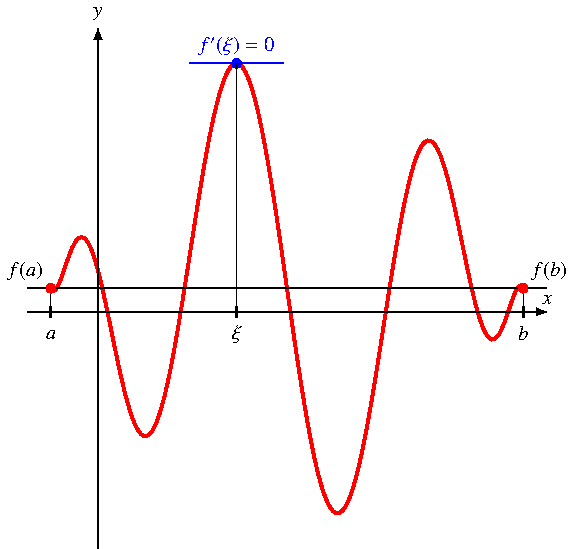
\includegraphics{chapters/30-interpolation/figures/rolle.pdf}
\caption{Satz von Rolle: eine nicht konstante differenzierbare Funktion,
die an den Enden eines Intervals den gleichen Funktionswert hat, hat im 
Inneren des Intervals eine Stelle $\xi$ mit Ableitung $0$.
\label{buch:figure:rolle}}
\end{figure}
Der Satz von Rolle erweitert den Zwischenwertsatz auf die Ableitung einer
differenzierbaren Funktion an (Abbildung~\ref{buch:figure:rolle}).

\begin{satz}[Rolle]
\label{buch:satz:rolle}
Sei $f$ eine auf dem Interval $[a,b]$ nicht konstante,
stetig differenzierbare Funktion
mit $f(a)=f(b)$, dann gibt es einen Punkt $\xi\in(a,b)]$ im Inneren
des derart, dass $f'(\xi)=0$.
\end{satz}

Der Satz von Rolle ist eine selbstverständlichkeit, wenn die Ableitung
$f'(x)$ stetig ist, doch dies wird nicht vorausgesetzt, es wird nur
verlangt, dass die Ableitung existiert.
Ausserdem macht der Satz eine Aussage darüber, dass die Zwischenstelle
$\xi$ im Inneren des Intervals sei.

\begin{proof}[Beweis]
Eine stetige Funktion hat auf dem kompakten Interval $[a,b]$ mindestens
ein Maximum und ein Minimum.
Da die Funktion nicht konstant ist, ist das Maximum oder das Minimum
von $f(a)$ verschieden.
Wir nehmen an $\xi\in[a,b]$ sei ein Maximum mit dieser Eigenschaft,
das Argument für das Minimum ist völlig analog.
Wegen $f(\xi)>f(a)$ ist $\xi$ ein Punkt im Inneren des Intervals,
also $\xi\in(a,b)$.

Wegen $f(\xi) \ge f(x)\forall x\in[a,b]$
folgt dann
\begin{align*}
f'(\xi) &= \lim_{h\to 0+}  \frac{f(\xi+h)-f(\xi)}{h} \le 0
\\
f'(\xi) &= \lim_{h\to 0-}  \frac{f(\xi+h)-f(\xi)}{h} \ge 0.
\end{align*}
Da $f$ differenzierbar ist, müssen diese beiden Grenzwerte übereinstimmen,
also ist $f'(\xi)=0$.
\end{proof}


\subsubsection{Nullstellen und der Satz von Rolle}
\begin{figure}
\centering
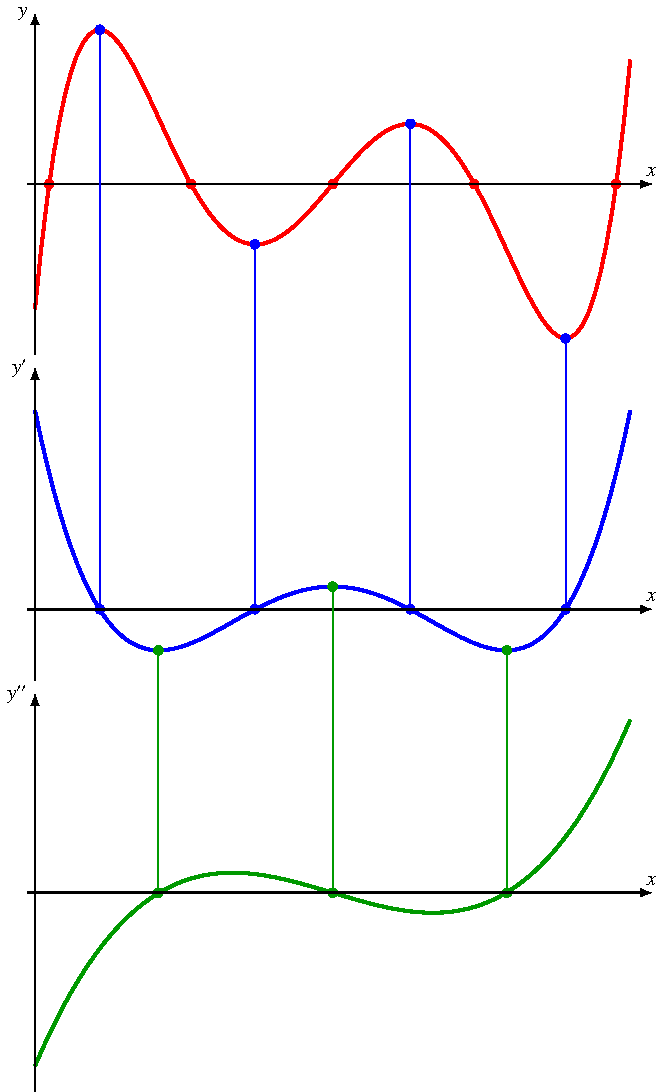
\includegraphics{chapters/30-interpolation/figures/nullstellen.pdf}
\caption{Schachtelung der Nullstellen von $f(x)$, $f'(x)$ und $f''(x)$.
Der Satz von Rolle~\ref{buch:satz:rolle} impliziert, dass sich zwischen zwei
Nullstellen von $f$ immer eine Nullstelle von $f'$ befindet, und
ebenso zwischen zwei Nullstellen von $f'$ eine von $f''$.
\label{buch:figure:nullstellen}}
\end{figure}

\begin{satz}
\label{buch:satz:nullstellen}
Ist $f$ eine differenzierbare Funktion auf dem Intervall $[a,b]$
mit Nullstellen 
\[
a=x_0 < x_1 < x_2 < \dots < x_{n-1} < x_n = b,
\]
die auf keinem Teilintervall $[x_i,x_{i+1}]$ konstant ist,
dann hat $f'$ im Inneren jedes Teilintervalls $[x_i, x_{i+1}]$
eine Nullstelle.
\end{satz}

Das Polynom 
\[
l(x) = (x-x_0)(x-x_1)\dots (x-x_{n-1})(x-x_n),
\]
welches für die Konstruktion des Interpolationspolynoms verwendet
wurde, hat genau die Nullstellen $x_0,x_1,\dots,x_{n-1},x_n$.
Nach dem Satz~\ref{buch:satz:nullstellen} muss es zwischen je
zwei aufeinanderfolgenden Nullstellen von $l$ eine Nullstelle der
Ableitung geben. 
Diese Situation ist in Abbildung~\ref{buch:figure:nullstellen}
für den Fall $l(x)=(x+2)(x+1)x(x-1)(x-2)$ dargestellt.

Die höheren Ableitungen $f^{(k)}$ haben ihre Nullstellen
natürlich auch wieder zwischen den Nullstellen der Ableitung $f^{(k-1)}$.
Die $n$-te Ableitung ist konstant und hat keine Nullstellen.

\begin{figure}
\centering
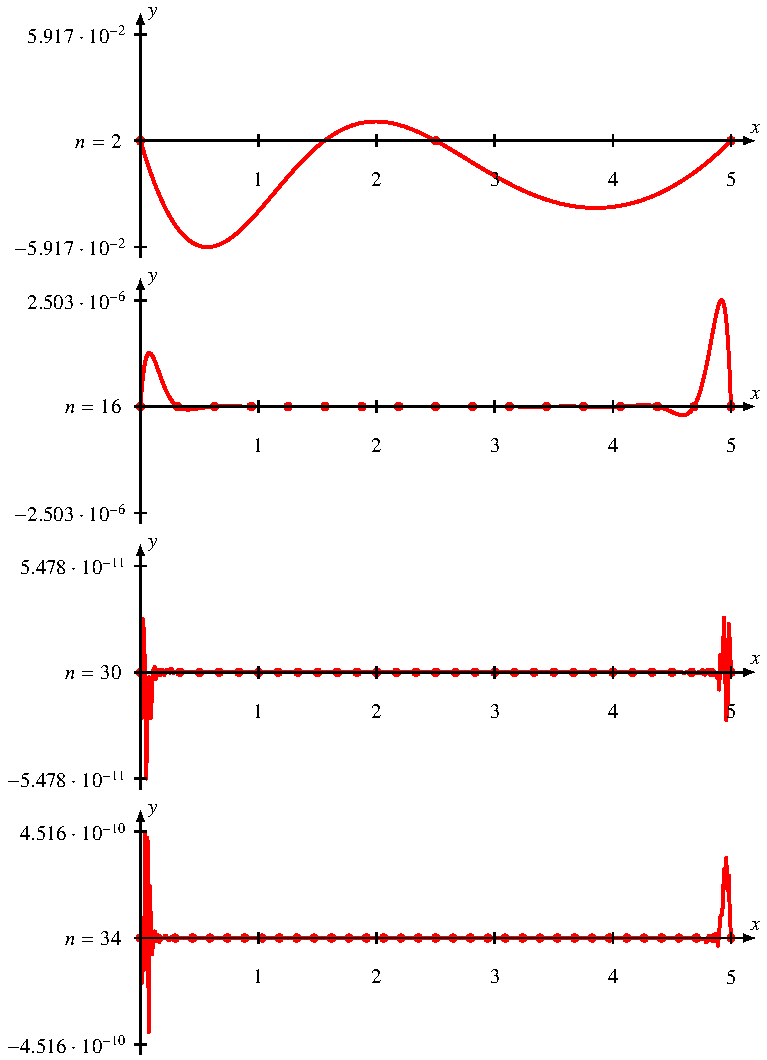
\includegraphics{chapters/30-interpolation/figures/norm.pdf}
\caption{Fehler des Lagrange-Interpolationspolynoms für die Funktion
$f(x)=e^{-x^2/2}/\sqrt{2\pi}$.
Der Fehler nimmt mit der Anzahl der Stützstellen bis $n=30$ ab, danach
wird die Berechnung instabil und der Fehler nimmt wieder zu.
\label{buch:figure:lagrangefehler}}
\end{figure}

\subsubsection{Der Mittelwertsatz der Differentialrechnung}
Der Satz von Rolle sagt etwas über die Nullstellen von der Ableitung
einer differenzierbaren Funktion.
Zwischen zwei Argumentwerten mit gleichem Funktionswert gibt es immer
eine Nullstelle der Ableitung.
Der Mittelwertsatz der Differentialrechnung verallgemeinert diese
Aussage auf beliebige Werte.

\begin{figure}
\centering
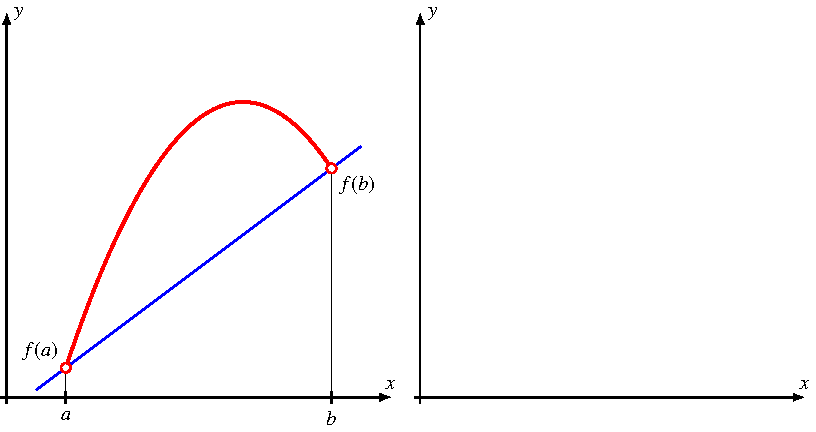
\includegraphics{chapters/30-interpolation/figures/mittelwertsatz.pdf}
\caption{Der Mittelwertsatz~\ref{buch:satz:mittelwertsatz} besagt, dass
die Sekante des Graphen einer differenzierbaren Funktion immer eine
Tangente mit der gleichen Steigung hat.
Diese Eigenschaft kann man auch für eine beliebige ebene Kurven
erwarten (rechts), dies ist der Inhalt des verallgemeinerten
Mittelwertsatzes~\ref{buch:satz:vmittelwertsatz}.
\label{buch:polynome:figure:mittelwertsatz}}
\end{figure}

\begin{satz}[Mittelwertsatz]
\label{buch:satz:mittelwertsatz}
Zu einer auf dem Intervall $[a,b]$ differenzierbaren Funktion $f(x)$ gibt
es immer ein $\xi\in[a,b]$ mit
\[
f'(\xi) = \frac{f(b)-f(a)}{b-a}
\]
(Abbildung~\ref{buch:polynome:figure:mittelwertsatz}).
\end{satz}

\begin{proof}[Beweis]
Man betrachtet die Funktion 
\[
g(x) = f(x) - \frac{f(b)-f(a)}{b-a}(x-a),
\]
sie hat an den Intervallenden die Werte
\begin{align*}
g(a) &= f(a) - \frac{f(b)-f(a)}{b-a}(a-a)=f(a),
\\
g(b) &= f(b) - \frac{f(b)-f(a)}{b-a}(b-a) = f(b) - \bigl(f(b)-f(a)\bigr) = f(a).
\end{align*}
Die Funktionswerte an den Intervallenden sind also gleich,
nach dem Satz~\ref{buch:satz:rolle} von Rolle hat also
die Ableitung $g'$ eine Nullstelle $\xi\in[a,b]$:
\[
g'(\xi) = f'(\xi) - \frac{f(b)-f(a)}{b-a} = 0
\quad
\Rightarrow
\qquad
f'(\xi) = \frac{f(b)-f(a)}{b-a}.
\qedhere
\]
\end{proof}

Die von Abbildung~\ref{buch:polynome:figure:mittelwertsatz} vermittelte
Intuition lässt sich auch für beliebige parametrisierte Kurven
$\gamma\colon[a,b]\to\mathbb R:\to\mapsto (x(t),y(t))$ in der Ebene
verallgemeinern (Abbildung~\ref{buch:polynome:figure:mittelwertsatz} rechts).
Sind die Punkte $A=(x(a),y(a))$ und $B=(y(a),y(b))$ verschieden,
so dass die Richtung von $A$ nach $B$ wohldefiniert ist, dann erwarten
wir einen Zwischenstelle $\xi$ mit einer Tangente mit derselben Richtung.

\begin{satz}
\label{buch:satz:mittelwertsatz2d}
Sei $\gamma\colon[a,b]\to\mathbb R:t\mapsto (x(t),y(t))$ eine
stetig differenzierbare ebene Kurve mit $|\dot{gamma}(t)|\ne 0$ für
alle $t\in[a,b]$ und $A=\gamma(a)\ne\gamma(b)=B$.
Dann gibt es ein $\xi\in[a,b]$ derart, dass $\dot{\gamma}(\xi)$ die gleiche
Richtung hat wie $\overrightarrow{AB}$.
\end{satz}

\begin{proof}[Beweis]
Zwei Vektoren haben die gleiche Richtung, wenn die Determinante
mit den Vektoren als Spaltenvektoren verschwindet.
Der Mittelpunkt der Strecke $AB$ ist
$M=(x_M,y_M) = (\frac12(x(a)+x(b)),\frac12(y(a)+y(b)))$.
Wir definieren die Funktion
\[
h(t)
=
\det(\overrightarrow{M\gamma(t)}, \overrightarrow{AB})
=
\biggl|
\begin{matrix}
x(t) - x_M & x(b)-x(a) \\
y(t) - y_M & y(b)-y(a)
\end{matrix}
\biggr|
\]
Da die Strecken $AB$ und $MA$ bzw.~$MB$ gleich sind, ist an den
Stellen $t=a$ und $t=b$ 
\[
h(a)
=
\det (\overrightarrow{MA},\overrightarrow{AB})
= 0
\qquad\text{and}\qquad
h(b)
=
\det (\overrightarrow{MB},\overrightarrow{AB})
=
0.
\]
Nach dem Satz von Rolle muss es daher ein $\xi\in[a,b]$ geben mit
\begin{equation}
0
=
h'(\xi)
=
\det(
\dot{\gamma}(\xi),
\overrightarrow{AB}
)
=
\biggl|
\begin{matrix}
x'(\xi) & x(b)-x(a) \\
y'(\xi) & y(b)-y(a)
\end{matrix}
\biggr|,
\label{buch:polynome:eqn:mittelwertsatz2d}
\end{equation}
was natürlich wieder bedeutet, dass die Tangente $\dot{\gamma}(\xi)$ 
parallel ist zur Strecke $AB$.
\end{proof}


\begin{satz}[Verallgemeinerter Mittelwertsatz]
\label{buch:satz:vmittelwertsatz}
Sind $x(t)$ und $y(t)$ stetig differenzierbare Funktionen auf dem Interval
$[a,b]$ derart, dass $x(a)\ne x(b)$ oder $y(a)\ne x(b)$ und ausserdem
$y'(t)\ne 0$ für $t\in[a,b]$.
Dann gibt es ein $\xi\in[a,b]$ mit
\[
\frac{y'(\xi)}{x'(\xi)}
=
\frac{y(b)-y(a)}{x(b)-x(a)}.
\]
\end{satz}

\begin{proof}[Beweis]
Die Bedingungen bedeuten, dass die die Kurve $\gamma(x(t),y(t))$
den Voraussetzungen des Satzes~\ref{buch:satz:mittelwertsatz2d}
genügt.
Es gibt daher einen Punkten $\xi\in[a,b]$ wo die Tangente
parallel zur Strecke $AB$ ist.
Nach~\label{buch:polynome:eqn:mittelwertsatz2d} bedeutet dies
\[
y'(\xi) \cdot (x(b)-x(a))
-
x'(\xi) \cdot (y(b)-y(a))
=0
\qquad\Rightarrow\quad
\frac{x'(\xi)}{y'(\xi)}
=
\frac{y(b)-y(a)}{x(b)-x(a)}.
\qedhere
\]
\end{proof}

Der Mittelwertsatz verspricht die Existenz eines Arguments $\xi\in[a,b]$,
gibt aber keinerlei Hinweise darauf, wie $\xi$ berechnet werden könnte. 
Ausserdem ist lässt sich der Satz in dieser Form nicht auf höherdimensionale
Situationen verallgemeinern.
In vielen Anwendungen des Mittelwertsatzes ist der genaue Wert von $\xi$
gar nicht nötig.
Meistens wird nur verwendet, dass die Ableitung eine Abschätzung dafür
gibt, wie gross der Unterschied zwischen $f(b)$ und $f(a)$ sein kann.
Dies kann zum Beispiel wie im folgenden Satz formuliert werden.

\begin{satz}
Für eine in $[a,b]$ stetig differenzierbare Funktion
$f\colon [a,b]\to\mathbb R^n$ gibt es ein $\xi\in[a,b]$ mit
\[
|f(b)-f(a)| \le |f'(\xi)|\cdot |b-a|.
\]
\end{satz}

\begin{proof}[Beweis]
\cite[(8.5.1)]{buch:dieudonne}
\end{proof}

Diese Form ist ausreichend, um zum Beispiel Fehlerabschätzungen in der
Numerik durchzuführen.

\subsubsection{Taylorreihe mit Lagrange-Restterm}
Die Ableitung $f'(a)$ einer Funktion $f(x)$ an der Stelle $a$ ist definiert
als die beste lineare Approximation
\[
f(x) = f(a) + f'(a)\cdot (x-a) + o(|x-a|).
\]
Der Mittelwertsatz besagt, dass
\[
f(x) = f(a) + f'(\xi) \cdot (x-a)
\]
für ein geeignetes $\xi\in[a,x]$.
Man kann also sagen, dass $f(a)$ eine Approximation für $f(x)$ mit einem
Fehler der Form $f'(\xi)\cdot(x-a)$ für ein geeignetes $\xi\in[a,x]$ ist.
Das Taylor-Polynom verallgemeinert diese Beobachtung auf eine Approximation
höherer Ordnung.

\begin{satz}
Sei $f(x)$ eine $n+1$-mal stetig differenzierbare Funktion in einer
Umgebung von $a$.
Dann ist das {\em Taylor-Polynom}
\begin{align*}
T_{a,n}f(x)
&=
f(a) + f'(a)\cdot (x-a) + f''(x)\frac{(x-a)^2}{2!} + f'''(x)\frac{(x-a)^3}{3!}
+\dots+f^{(n)}(a)\frac{(x-a)^n}{n!}
\\
&=
\sum_{k=0}^n
f^{(k)}(a) \frac{(x-a)^k}{k!}
\end{align*}
eine Approximation von $f(x)$ derart, dass
\[
f(a)=T_{a,n}f(a),\quad
f'(a)=T_{a,n}f'(a),\quad
f''(a)=T_{a,n}f''(a),\quad
\dots,\quad
f^{(n)}(a)=T_{a,n}f^{(n)}(a).
\]
Ausserdem gibt es einen Wert $\xi\in[a,x]$ derart, dass der Fehler
\[
R_{n,a}f(x)
=
f(x) - T_{n,a}f(x)
=
f^{(n+1)}(\xi)\frac{(x-a)^{n+1}}{(n+1)!}
\]
ist.
\end{satz}
\index{Taylor-Polynom}
$R_{n,a}f(x)$ heisst das {\em Lagrange-Restglied} des Taylor-Polynoms.

\begin{proof}[Beweis]
Zunächst kann die Behauptung über die Ableitungen von $T_{n,a}f(x)$ durch
die Rechnung
\begin{align*}
T_{n,a}f'(x)
&=
f'(a) + f''(a) \cdot (x-a) + f'''(a)\frac{(x-a)^2}{2!} + \dots
&&\Rightarrow&
T_{n,a}f'(a) 
&=
f'(a)
\\
T_{n,a}f''(x)
&=
f''(a) + f'''(a) \cdot (x-a) + \dots
&&\Rightarrow&
T_{n,a}f''(a) 
&=
f''(a)
\\
&\;\vdots&&&&\;\vdots
\\
T_{n,a}f^{(n)}(x)
&=
f^{(n)}(a)
&&\Rightarrow&
T_{n,a}f^{(n)}(a)
&=
f^{(n)}(a)
\end{align*}
direkt bestätigt werden.
Daraus folgt, dass die Funktion $g(x) = f(x) - T_{n,a}f(x)$ die Eigenschaft
\begin{equation}
g(a) = g'(a) = g''(a) = \dots = g^{(n)}(a)=0
\label{buch:taylor:gabl}
\end{equation}
hat.
Es muss als nur gezeigt werden, dass es unter den Voraussetzungen
\eqref{buch:taylor:gabl} eine Zahl $\xi$ gibt derart, dass
\[
g(x) = g^{(n+1)}(\xi)\frac{(x-a)^{n+1}}{(n+1)!}
\]
gilt.
Der Fall $n=0$ ist der Mittelwertsatz~\ref{buch:satz:mittelwertsatz}.

Für $n>0$ kann die Behauptung mit vollständiger Induktion bewiesen werden.
Sei also bereits bewiesen, dass für eine Funktion, deren Ableitungen bis
zur Ordnung $n-1$ an der Stelle $a$ verschwinden, eine Zahl $\xi\in[a,x]$
existiert mit
\[
g(x) = g^{(n)}(\xi)\frac{(x-a)^n}{n!}
\]
und müssen jetzt zeigen, dass dies auch für $n+1$ gilt.

Wir müssen $g(x)$ mit $(x-a)^{n+1}$ vergleichen und untersuchen
dazu den Quotienten
\[
\frac{g(x)}{(x-a)^{n+1}}.
\]
Zur Abkürzung schreiben wir $h(x) = (x-a)^{n+1}$, es ist also der
Quotient 
\[
\frac{g(x)}{h(x)}
=
\frac{g(x)-g(a)}{h(x)-h(a)}
\]
zu berechnen.
Nach dem verallgemeinerten Mittelwertsatz~\ref{buch:satz:vmittelwertsatz}
gibt es $\xi_1\in[a,x]$ mit
\[
\frac{g'(\xi_1)}{h'(\xi_1)}
=
\frac{g(x)-g(a)}{h(x)-h(a)}.
\]
Da die Ableitung $h'(x)=(n+1)(x-a)^n$ ist, folgt
\begin{equation}
\frac{g'(\xi_1)}{h'(\xi_1)}
=
\frac{g'(\xi_1)}{(n+1) (\xi_1-a)^n}
=
\frac{g(x)-g(a)}{h(x)-h(a)}
=
\frac{g(x)}{(x-a)^{n+1}}.
\label{buch:taylor:eqn1}
\end{equation}
Die Ableitungen der Ordnung $\le n-1$ der Funktion $g'(x)$ verschwinden
im Punkt $a$, nach Induktionsvoraussetzung gibt es also ein $\xi$ derart,
dass
\[
g'(\xi_1)
=
(g')^{(n)}(\xi) \frac{(\xi_1-a)^{n}}{n!}
=
g^{(n+1)}(\xi)\frac{(\xi_1-a)^n}{n!}
\]
gilt.
Setzt man dies in \eqref{buch:taylor:eqn1} ein, erhält man
\[
\frac{g(x)}{(x-a)^{n+1}}
=
\frac{g'(\xi_1)}{(n+1)(\xi_1-a)^n}
=
g^{(n+1)}(\xi)\frac{(\xi_1-a)^n}{n!} \frac{1}{(n+1)(\xi_1-a)^n}
=
g^{(n+1)}(\xi)\frac{1}{(n+1)!}.
\]
Durch Multiplikation mit $(x-a)^{n+1}$ erhalten wir
\[
g(x) = g^{(n+1)}(\xi)\frac{(x-a)^{n+1}}{(n+1)!}.
\]
Damit ist der Induktionsschritt vollzogen und die Restwertformel bewiesen.
\end{proof}

\begin{beispiel}
Die Funktion $f(x)=x^N$ hat an der Stelle $a=0$ verschwindende
Ableitungen bis zur Ordnung $N-1$.
Das Taylor-Polynom $T_{0,n}f(x)$ der Ordnung $n$ dieser Funktion
verschwindet daher für $n<N$.
Nach der Restformel des Taylor gibt es Zahlen $\xi_n$ derart
\begin{align*}
R_{n,0}f(x)
=
f(x)
&=
x^N
= 
f^{(n+1)}(\xi_n) \frac{x^{n+1}}{(n+1)!}
\\
&=
\frac{
N\cdot(N-1)\cdot(N-2)\cdot\dots\cdot(N-n)
}{
1\cdot 2 \cdot 3 \cdot\dots \cdot (n+1)
}
\xi_n^{N-n-1} 
=
\binom{N}{n+1} \xi_n^{N-n-1}
\\
\Rightarrow\qquad
\xi_n
&=
\binom{N}{n+1}^{\frac{-1}{N-n-1}} x^{\frac{N}{N-n-1}}.
\qedhere
\end{align*}
\end{beispiel}

Im Hinblick auf die nachfolgende Diskussion des Fehlers des
Interpolationspolynoms formulieren wir dies noch als eine
Fehlerabschätzung.
Das Taylor-Polynom approximiert die Funktion $f(x)$ durch ein
Polynom vom Grad $n$.
Der Fehler des Taylor-Polynoms ist
\[
|f(x) - T_{n,a}f(x)|
=
\biggl|
f^{(n+1)}(\xi)
\frac{(x-a)^{n+1}}{(n+1)!}
\biggr|
=
|f^{(n+1)}(\xi)|\cdot
\biggl|
\frac{(x-a)^{n+1}}{(n+1)!}
\biggr|
\le
\max_{\xi\in [a,x]} |f^{(n+1)}(\xi)|
\biggl|
\frac{(x-a)^{n+1}}{(n+1)!}
\biggr|,
\]
er ist also beschränkt einerseits durch ein Polynom mit Grad $n+1$
und den grössten Wert der $(n+1)$-te Ableitung im Intervall $[a,x]$.
Die Fehlerformel für das Interpolationspolynom wird von der genau
gleichen Art sein.

\subsubsection{Fehler des Lagrange-Interpolationspolynoms}
Der folgende Satz gibt vollständige Auskunft über den Fehler des
Interpolationspolynoms.

\begin{satz}
\label{buch:satz:lagrangefehler}
Sei $p$ ein Polynom vom Grad $n$, welches mit der $n+1$-mal differenzierbaren
Funktion $f$ an den $n+1$ Stellen
\[
a = x_0 < x_1 < x_2 < \dots  < x_{n-1} < x_n=b
\]
übereinstimmt.
Dann gibt es für jedes $x\in[a,b]$ ein $\xi_x\in [a,b]$ mit
\begin{equation}
f(x) - p(x) = \frac{f^{(n+1)}(\xi_x)}{(n+1)!} l(x).
\label{buch:equation:polyfehler}
\end{equation}
\end{satz}

\begin{proof}[Beweis]
An den Stützstellen $x_i$ ist $f(x_i)-p(x_i)=0$ und $l(x_i)=0$, die
Gleichung~\eqref{buch:equation:polyfehler} ist also trivialerweise
erfüllt.

Sei jetzt also $x\in[a,b]$ verschieden von allen $x_i$.
Da $l(x)\ne 0$ ist, gibt es eine Zahl $c$ derart, dass
\begin{equation}
f(x)-p(x)=cl(x)
\qquad\Leftrightarrow\qquad
f(x)-p(x)-cl(x)=0.
\label{buch:equation:polyfehler1}
\end{equation}
Die Funktion $g(x)=f(x)-p(x)-cl(x)$ verschwindet in allen Stützstellen $x_i$
und zusätzlich auch noch im Punkt $x$, sie hat also $n+1$ Nullstellen.

Nach dem Nullstellen-Schachtelungssatz~\ref{buch:satz:nullstellen}
hat die $n+1$ Ableitung von $g$ eine Nullstelle im Intervall.
Es gibt also eine Zahl $\xi_x\in[a,b]$ mit $g^{(n+1)}(\xi_x)=0$.

Da $p$ Grad $n$ hat, ist die $n+1$-te Ableitung $0$.
Das Polynom $l(x)$ hat die Form
\[
l(x) = x^{n+1} -(x_0+x_1+\dots+x_{n-1}+x_n)x^{n-1} + \dots + (-1)^{n+1}x_0x_1\dots x_{n-1}x_n,
\]
seine $n+1$-Ableitung ist die Konstanten $(n+1)!$.

Die Folgerung $g^{(n+1)}(\xi_x)=0$ wird damit zu
\[
0 = f^{(n+1)}(\xi_x) -c (n+1)!
\qquad\Rightarrow\quad
c=\frac{f^{(n+1)}(\xi_x)}{(n+1)!}.
\]
Einsetzen in \eqref{buch:equation:polyfehler1} ergibt
\[
f(x)-p(x) = cl(x)=\frac{f^{(n+1)}(\xi_x)}{(n+1)!} l(x),
\]
wie behauptet.
\end{proof}

Dieser Satz erlaubt den Fehler eines Interpolationspolynoms abzuschätzen,
wenn die $n+1$-te Ableitung der Funktion $f$ bekannt ist.
Wir bezeichnen mit
\[
\|g\| = \sup_{a\le x\le b} |g(x)|
\]
die {\em Supremun-Norm} der Funktion $g$ im Intervall $[a,b]$.
\index{Supremum-Norm}

\begin{korollar}
\label{buch:korollar:interpolationsfehler}
Ist $p$ ein Interpolationspolynom vom Grad $n$, welches mit der Funktion
$f$ in den Stellen $a=x_0<x_1<\dots <x_{n+1}<x_n=b$ übereinstimmt, dann
ist 
\[
|f(x)-p(x)| \le \frac{\|f^{(n+1)}\|}{(n+1)!} |l(x)|.
\]
\end{korollar}

Der Fehler des Interpolationspolynoms vom Grad $n$ ist also beschränkt
durch das Polynom $l(x)$ vom Grad $n+1$ und den grössten Wert der
$(n+1)$-ten Ableitung von $f(x)$.

\begin{beispiel}
\begin{figure}
\centering
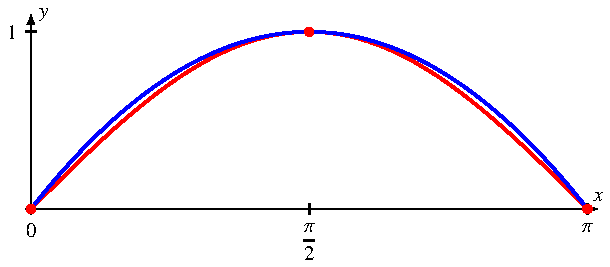
\includegraphics{chapters/30-interpolation/figures/sin.pdf}
\caption{Interpolation der Funktion $f(x)=\sin x$ mit nur drei 
Stützstellen $x_0=0$, $x_1=\frac{\pi}2$ und $x_2=\pi$.
Der Fehler ist deutlich kleiner als die Abschätzung mit
Satz~\ref{buch:satz:lagrangefehler} erwarten lässt.
\label{buch:figure:sin}}
\end{figure}
Die Funktion $f(x)=\sin x$ soll mit den Stützstellen $x_0=0$, $x_1=\frac{\pi}2$
und $x_2=\pi$ interpoliert werden.
Das Interpolationspolynom ist ein quadratisches Polynom mit Nullstellen
$x_0$ und $x_2$, der Funktionswert bei $x_1$ muss $1$ sein.
Man kann sich davon überzeugen, dass das Polynom
\[
p(x) = \frac{4}{\pi^2} x(\pi -x )
\]
diese Eigenschaft hat.
Wie gross ist der Fehler dieses Interpolationspolynoms?

Die dritten Ableitungen der Funktion $f(x)=\sin x$ sind, bekannt, es ist
$f^{(3)}(x)=-\cos x$.
Der Betrag von $f^{(3)}(x)$ wird also nie grösser als $1$.
Es folgt, dass
\[
|f(x)-p(x)| \le \frac{1}{3!} l(x)
=
\frac16 |x(x-{\textstyle\frac{\pi}2})(x-\pi)|
\]
Die Ableitung des Polynoms auf der rechten Seite hat Nullstellen bei
$\frac{\pi}2 \pm \frac{\pi}{2\sqrt{3}}$,
durch Einsetzen erhält man den maximalen Wert
\[
\|f^{(3)}\|
=
\frac{\pi^3}{12\sqrt{3}}\simeq 1.49179.
\]
Wir schliessen, dass das Interpolationspolynom niemals um mehr als $0.24863$
vom Funktionswert abweichen kann.
\end{beispiel}

%
% Tschebyscheff Interpolation
%
\subsection{Wahl der Stützstellen und Tschebyscheff-Interpolationspolynom
\label{buch:section:interpolation:tschebyscheff}}
Das Korollar~\ref{buch:korollar:interpolationsfehler} besagt, dass der
Fehler des Interplationspolynom durch den Betrag von $l(x)$ begrenzt
ist.
Für äquidistante Stützstellen mit Abstand $h$ kann man beobachten,
dass die Oszillationen des Polynoms $l(x)$ gegen den Rand des Intervalls
immer grösser werden.
Für einen Punkte in der Mitte jedes Teilintervalls ist $h/2$ der kleinste
mögliche Faktor in $l(x)$. 
Den grössten Faktor findet man für $x$ im ersten oder letzten Teilinterval,
er ist $b-a-h$.
Ausserdem treten mehrere ähnlich grosse Faktoren auf.
Für $x$ in einem Intervall nahe $(a+b)/2$ sind die Faktoren
dagegen nur halb so gross.

Die Oszillationen können verkleinert werden, wenn man dafür sorgt, dass
mit grösserem Abstand von der Mitte des Intervalls der Abstand der
Stützstellen ebenfalls verkleinert.
Dies garantiert, dass neben den grossen Faktoren in der Nähe von $b-a$ 
auch wesentlich kleinere Faktoren auftreten, so dass die extremen Werte
nahe den Intervallenden vergleichbar mit den Werten im Inneren des
Intervalls werden.

\begin{figure}
\centering
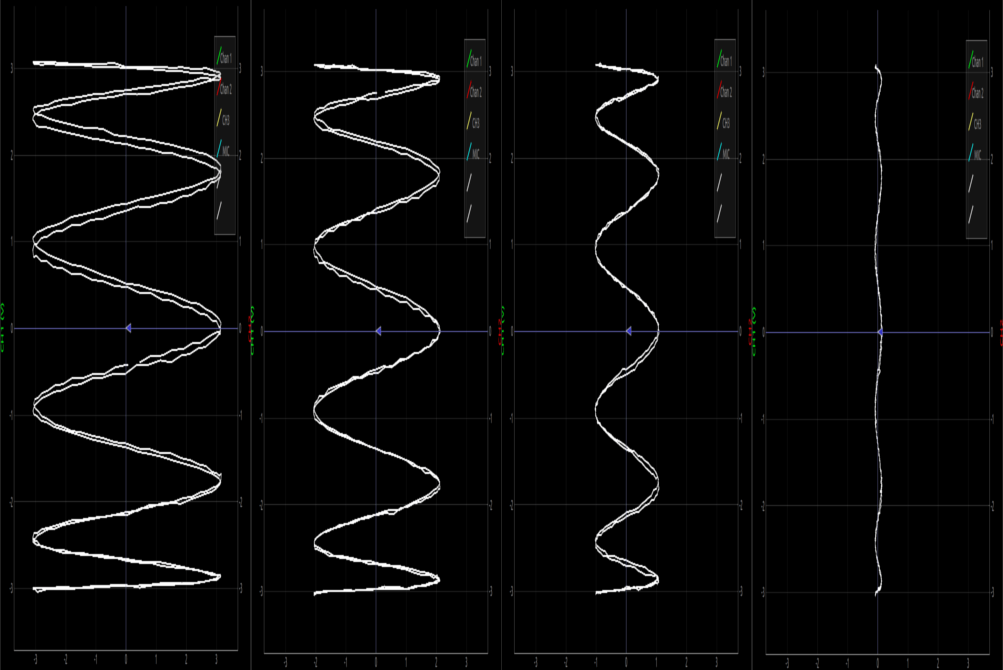
\includegraphics[width=\hsize]{chapters/30-interpolation/figures/lissajous.jpg}
\caption{Diese Lissajous-Figur suggeriert eine mögliche Lösung für eine 
Interpolationspolynom mit besonders kleinem Fehler.
Wenn sich diese Kurve als Polynom ausdrücken lässt, bleibt der Fehler über
das ganze Definitionsinterval gleichmässig beschränkt.
\label{buch:figure:lissajous}}
\end{figure}

Die beste Approximation durch ein Interpolationspolynom kann man also
erwarten, wenn $l(x)$ im Interval $[a,b]$ keine besonders grossen Werte
annimmt.
Eine Funktion ähnlich wie $\sin x$ oder $\cos x$, die unendlich viele
Extremewerte $\pm 1$ haben, würde dieses Kriterium erfüllen, aber
$\sin x$ und $\cos x$ sind keine Polynome.
Sie sind auch auf auf einem viel grösseren Interval als nötig definiert,
nämlich ganz $\mathbb R$.
Ein verwandtes Beispiel sind Lissajous-Figuren,
Abbildung~\ref{buch:figure:lissajous} suggeriert, dass eine geeignete
Lissajous-Figur als Graph für ein Interpolationspolynom mit sehr
geringem Fehler dienen könnte, wenn man sie als Polynom darstellen kann.
Eine solche Lissajous-Figur entsteht als Kurve
$t\mapsto (\cos t, \cos nt)$ oder eine anderes trigonometrisches
Polynom als zweite Komponente.
Es stellt sich also die Frage, ob $\cos nt$ als Polynom in $z=\cos t$
ausgedrückt werden kann.

Sei also
\[
T_n(z)
=
T_n(\cos t)
= 
\cos nt.
\]
Für kleine $n$ kann man unmittelbar verifizieren, dass $T_n(z)$ ein
Polynom ist:
\begin{equation}
\begin{aligned}
T_0(z) &= 1,\\
T_1(z) &= z,\\
T_2(z) &= \cos 2t = 2\cos^2 t-1 = 2z^2 -1
\quad\text{und}
\\
T_3(z) &= \cos 3t = 4\cos^3 t - 3\cos t = 4z^3-3z.
\end{aligned}
\label{buch:tschebyscheff:erste}
\end{equation}
Aus den Additionstheoremen für den Kosinus folgt die Formel für die
Summe von zwei Konsinus-Funktionen
\begin{align}
\cos (n+1)t + \cos(n-1)t
&=
2 \cos \frac{(n+1)t + (n-1)t}2 \cos \frac{(n+1)t -(n-1)t}2
=
2\cos nt \cos t
\notag
\\
T_{n+1}(z)+T_{n-1}(z)&=2zT_n(z)
\notag
\\
T_{n+1}(z) &= 2zT_n(z) - T_{n-1}(z).
\label{buch:tschebyscheff:rekursion}
\end{align}
Wenn $T_n(z)$ und $T_{n-1}(z)$ Polynome sind, dann ist auch $T_{n+1}(z)$
ein Polynom.
Aus den bereits gekannten Polynomen~\eqref{buch:tschebyscheff:erste} und
der Rekursionsformel~\eqref{buch:tschebyscheff:rekursion} folgt jetzt mit
vollständiger Induktion, dass alle $T_n(z)$ Polynome sind.
Sie heissen {\em Tschebyscheff-Polynome}.
\index{Tschebyscheff-Polynome}
Die Rekursionsformel kann dazu verwendet werden, die Polynome explizit
zu berechnen.
Zum Beispiel folgt für die nächsten paar Polynome
\begin{align*}
T_4(z) &= 8z^4-8z^2 + 1,
\\
T_5(z) &= 16z^5-20z^3+5z \quad\text{und}
\\
T_6(z) &= 32z^6-48z^4+18z^2-1.
\end{align*}
Da das Interpolationspolynom den führenden Koeffizienten $1$ hat,
muss $l(z) = 2^{1-n}T_n(z)$ gewählt werden.

Die Polynome $T_n(z)$ sind eigentlich nicht nötig, da für die Konstruktion
des Interpolationspolynoms nur die Nullstellen nötig sind.
Wegen $T_n(z)=\cos nt$ liegt eine Nullstelle genau dann vor, wenn
$nt = \frac{\pi}2 + k\pi$, $k\in\mathbb Z$.
Die zugehörigen Werte von $z$ sind
\[
z_k
=
\cos t = \cos\frac{\pi(2k+1)}{2n}.
\]
In Abbildung~\ref{buch:figure:tschebyscheff-vergleich} sind 
die Polynome $2^{n-1}l(x)$ vom Grad $n$ oben für äquidistante Stützstellen
und unten für Tschebyscheff-Stützstellen im Vergleich dargestellt.
Wie in der Einleitung zu diesem Abschnitt angekündigt, oszillieren die
Polynome für äquidistante Stütztstellen nahe den Intervallenden.
Für Tschebyscheff-Stützstellen wird $2^{n-1}l(x)$ betragsmässig nie
grösser als $1$.
\begin{figure}
\centering
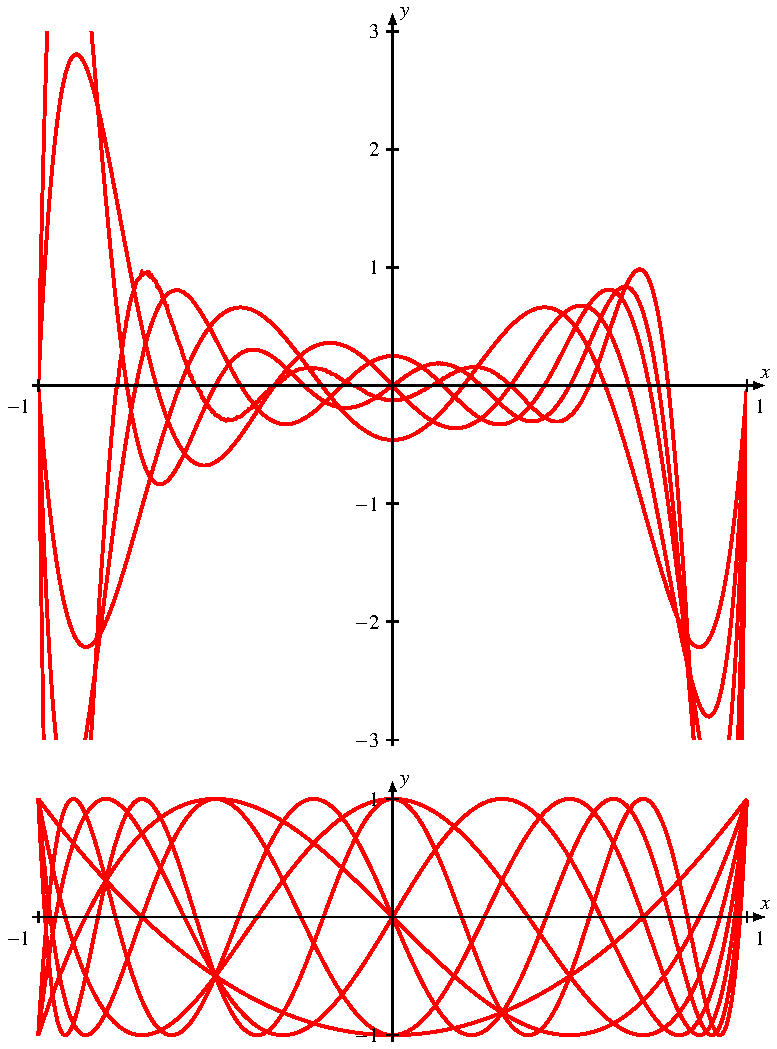
\includegraphics{chapters/30-interpolation/figures/vergleich.pdf}
\caption{Vergleich der Oszillationen bei äquidistanten Stützstellen (oben)
und bei Tschebyscheffstützstellen.
Damit die Abweichungen sichtbar werden, sind die Polynome $l(x)$ vom Grad
$n$ mit dem Faktor $2^{n-1}$ skaliert.
Bei Verwendung von Tscheby\-scheff-Stützstellen wächst $2^{n-1}l(x)$
nie über $1$ an, während bei äquidistanten Stützstellen die in der
Einleitung zu diesem Abschnitt diskutierten Oszillationen nahe den
Intervallenden auftreten.
\label{buch:figure:tschebyscheff-vergleich}}
\end{figure}

\begin{figure}
\centering
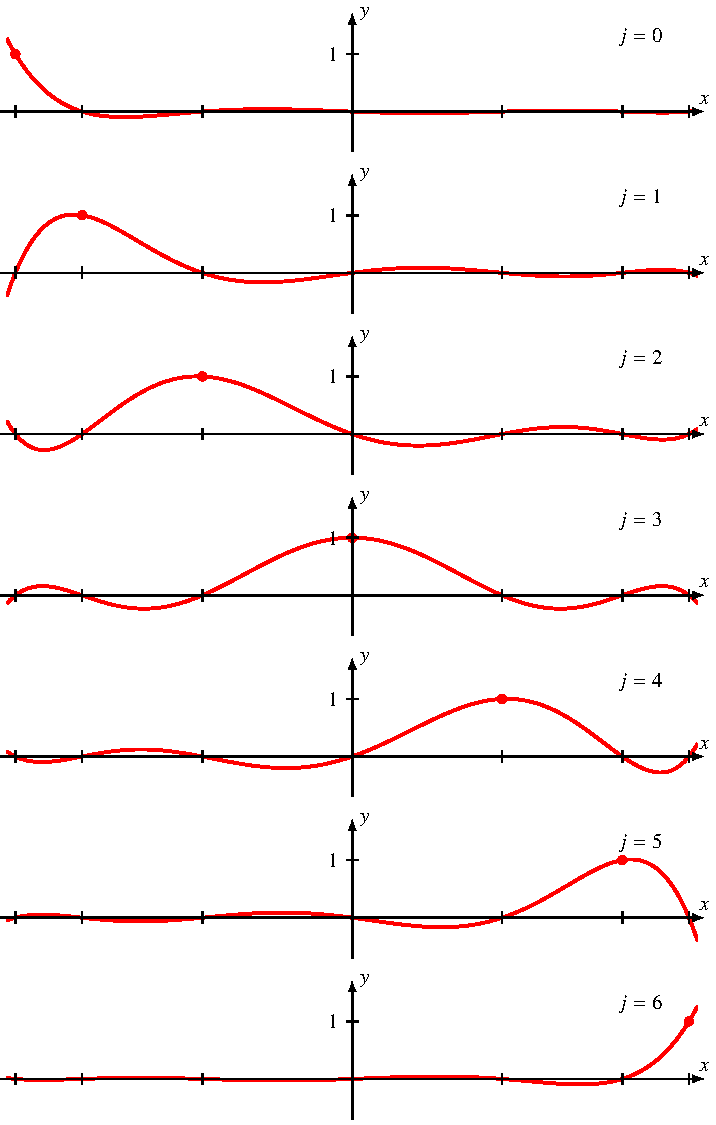
\includegraphics{chapters/30-interpolation/figures/tschebasis.pdf}
\caption{Basisinterpolationspolynome vom Grad 7 für
Tschebyscheff-Stützstellen
\label{buch:figure:tschebyscheffbasis}}
\end{figure}
Abbildung~\ref{buch:figure:tschebyscheffbasis} zeigt die Basispolynome
vom Grad 7 $l_j(x)$ für Tschebscheff-Stütztstellen.
Da bei Verwendung von Tschebyscheff-Stützstellen die Polynome $l(x)$
keine ausgeprägten Oszillationen an den Intervallenden aufweisen, 
sind auch die Basispolynome $l_j(x)$ vor allem in der Nähe der
jeweiligen Stützstelle $x_j$ wesentlich von $0$ verschieden.

\begin{figure}
\centering
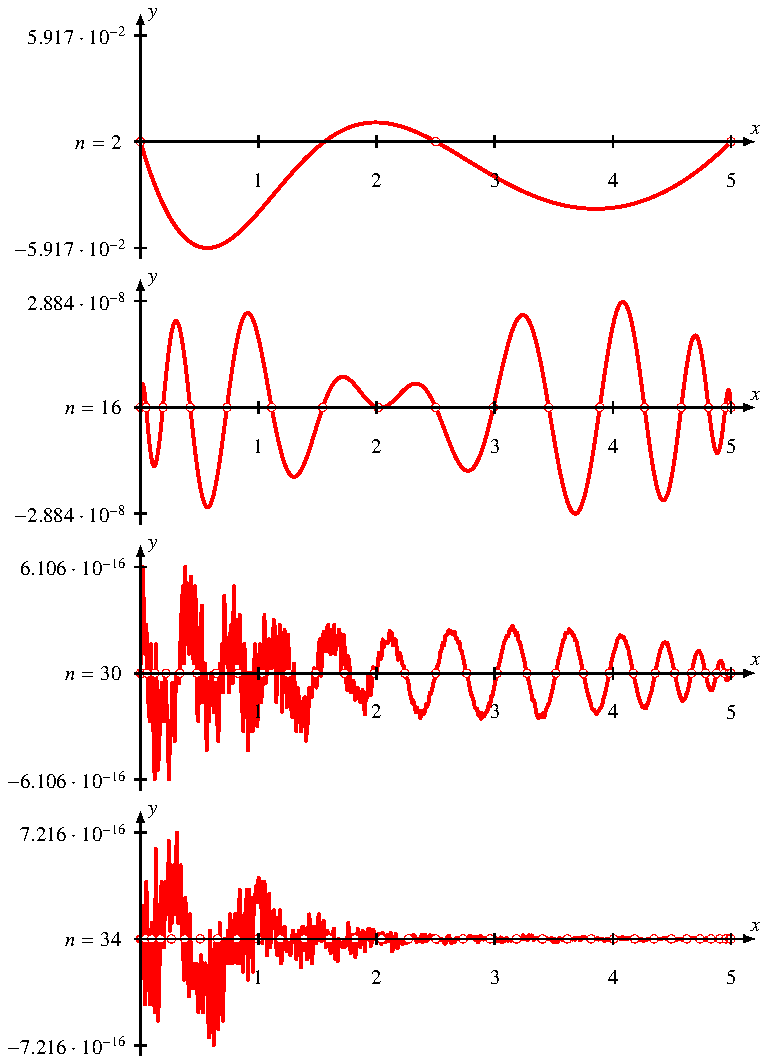
\includegraphics{chapters/30-interpolation/figures/tscheb.pdf}
\caption{Fehler des Interpolationspolynomes für die Funktion
$f(x)=e^{-x^2/2}/\sqrt{2\pi}$ mit Stützstellen nach Tschebyscheff.
Der Fehler bleibt über das ganze Intervall gleichmässig.
Für eine grosse Zahl von Stützstellen erreicht die Interpolation die
Maschienengenauigkeit.
\label{buch:figure:tschebyschefffehler}}
\end{figure}





